\documentclass[12pt,a4paper]{article}
    \usepackage[T2A]{fontenc}
    \usepackage[utf8]{inputenc}
    \usepackage[russian]{babel}
    \usepackage{amsmath}
    \usepackage{amssymb}
    \usepackage{graphicx}
    \usepackage{floatrow}
    \usepackage{booktabs}
    \usepackage{wrapfig}
    \usepackage{lipsum}
    \usepackage{subcaption}
    \usepackage{fancyhdr}
    \usepackage{mathrsfs}
    \usepackage{tikz}

    \usepackage{graphicx, scalerel}
    \usepackage[warn]{mathtext}
    \usepackage{indentfirst}
    \usepackage[margin = 25mm]{geometry}
    \usepackage{caption}
    \usepackage{multirow}
    \usepackage{gensymb}
    
    \newcommand{\figref}[1]{(См. рис. \ref{#1})}
    \newcommand{\secref}[1]{(См. раздел. \ref{#1})}
    
    \newcommand{\e}[1]{\text{$\cdot10^{#1}$}}
    
    \pagestyle{fancy}
    \fancyhead{}
    \fancyhead[L]{Работа 5.1.3}
    \fancyhead[R]{}
    \fancyfoot[C]{\thepage}
    
    \author{\normalsize Выполнил: Голубович Тимур, группа Б01-110 \\
    	\normalsize 08.11.2023}
    \date{}

    \usepackage{float}
    \restylefloat{table}
    \title{
    	\large Отчет о выполнении лабораторной работы 5.1.3 \\
    	\Large Эффект Рамзауэра
     }

    \begin{document}
\maketitle

\section*{Цель работы}

\textbf{Цель работы:} исследовать энергетическую зависимость вероятности рассеяния электронов на атомах газа, определить энергии электронов, при которых наблюдается его <<просветление>> и оценить размер его внешней электронной оболочки.

\section*{Оборудование и приборы}

Источник  $\gamma$-квантов со свинцовым коллиматором; набор поглотителей из различных материалов; сцинтилляционныйй счётчик; пересчётный прибор.
	
\section*{Теоретическое введение}

\begin{wrapfigure}{R}{0.4\textwidth}
		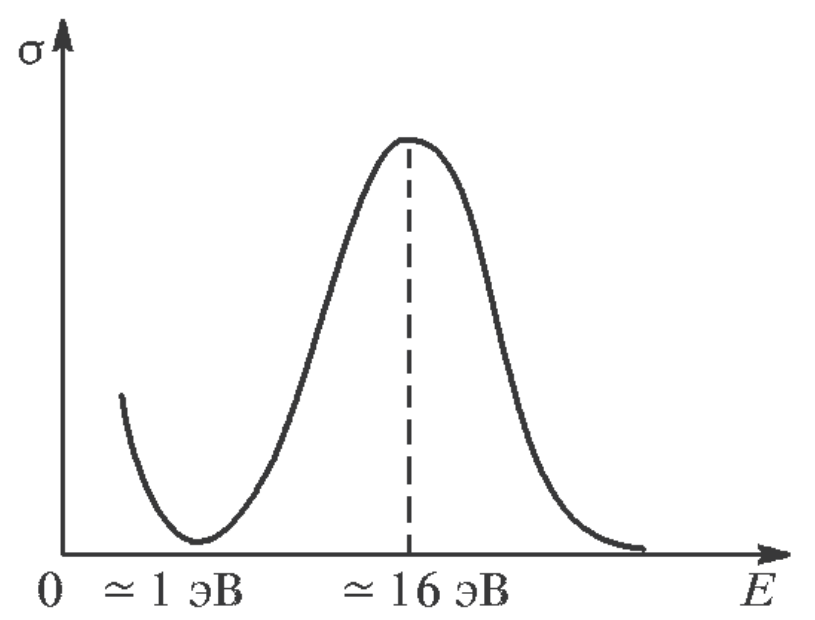
\includegraphics[width=0.8\textwidth]{res/2.png}
		\caption{Качественная картина результатов измерения упругого рассеяния электронов в аргоне}
	\end{wrapfigure}


	По мере уменьшения энергии электрона от нескольких десятков электрон-вольт поперечное сечение его упругого рассеяния растет, как это и следует из очень простых рассуждений: чем меньше скорость электрона, тем медленнее он «проскакивает» мимо атома, тем больше время взаимодействия электронов с атомом и, тем самым, больше вероятность этого взаимодействия, т. е. сечение реакции. Однако в эксперименте Рамзауэра с аргоном наблюдалось, что при энергиях меньше электронов 16 эВ сечение начинает уменьшаться, а при $E \simeq 1$ эВ практически равно нулю, т. е. аргон становится прозрачным для электронов. При дальнейшем уменьшении энергии электронов сечение рассеяния опять начинает возрастать. Объяснение этого эффекта потребовало учета волновой природы электронов.
	
	Пучок электронов, вылетая из накаленного катода $K$, проходит ускоряющую разность потенциалов $V$, приложенную между катодом и электродом Э, и приобретает тем самым энергию $E = mv^2/2 = eV$.
	\begin{wrapfigure}{L}{0.4\textwidth}
		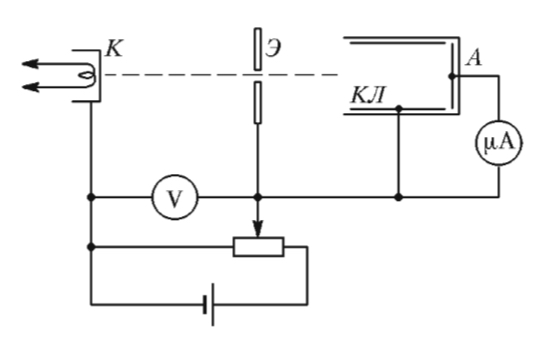
\includegraphics[width=0.8\textwidth]{res/1.jpg}
		\caption{Схема установки для измерения сечения рассеяния электронов в газах}
	\end{wrapfigure}

	Внутри атома потенциальная энергия налетающего электрона $U$ отлична от нуля, скорость электрона изменяется, становясь равной $v'$ в соответствии с законом сохранения энергии:
	\begin{equation}
		E = \frac{mv^2}{2} = \frac{mv'^2}{2} + U,
	\end{equation}
	а значит, изменяется и длина его волны де Бройля. Таким образом, по отношению к электронной волне атом ведет себя как преломляющая среда с относительным показателем преломления
	\begin{equation}
		n = \frac{\lambda}{\lambda'} = \sqrt{1-\frac{U}{E}}.
	\end{equation}

	Уравнение Шредингера в случае прохождении частицы с энергией $E$ над потенциальной ямой шириной $l$ и глубиной $U_0$:

    \begin{flalign}
        \psi'' + k^2 \psi = 0, \;\;\;\;\;\;\;\;\;\;\;\;\;\;\;\;\;\;\;\;\;\;\;\;\;\;\;\;\;\;\;\;\;\;\;\\
            \text{ где } k^2 = \begin{cases}
            k_1^2 = \frac{2mE}{\hbar^2} \text{ в областях вне ямы;} \\
            k_2^2 = \frac{2m(E + U_0)}{\hbar^2} \text{ в области ямы.}
        \end{cases} 
    \end{flalign}

	Коэффициент прохождения равен отношению квадратов амплитуд прошедшей и падающей волн и определяется выражением
	\begin{equation}
		D = \frac{16 k_1^2 k_2^2}{16 k_1^2 k_2^2 + 4(k_1^2 - k_2^2)^2 \sin^2{(k_2 l)}}
	\end{equation}
	
	Таким образом, коэффициент прохождения электронов максимален при условии
	\begin{equation}
		k_2 l = \sqrt{\frac{2m(E + U_0)}{\hbar^2}}l = \pi n, \; n = 1, 2, 3, ...
		\label{En}
	\end{equation}
	
	Аналогично, условия на первые максимум и минимум соответственно:
	\begin{equation}
		2l = \frac{h}{\sqrt{2m(E_1 + U_0)}}
		\label{E1}
	\end{equation}
	\begin{equation}
		2l = \frac{3}{2}\frac{h}{\sqrt{2m(E_2 + U_0)}}
		\label{E2}
	\end{equation}
	
	Решая совместно эти два уравнения, можно исключить $U_0$ и найти эффективный размер атома $l$:
	\begin{equation}
		l = \frac{h\sqrt{5}}{\sqrt{32m(E_2 - E_1)}}.
		\label{E2E1}
	\end{equation}

	Из этих же формул можно также по измеренным величинам $E_1$ и $E_2$ рассчитать эффективную глубину потенциальной ямы атома:
	\begin{equation}
		U_0 = \frac{4}{5}E_2 - \frac{9}{5}E_1.
		\label{U_0}
	\end{equation}
 	
 
\section*{Экспериментальная установка}
	
В нашей работе для изучения эффекта Рамзауэра используется тиратрон ТГ3-01/1.3Б, заполненный инертным газом. Схематическое изображение тиратрона и его конструкция приведены на рис. 3.
	
	\begin{wrapfigure}{R}{0.4\textwidth}
		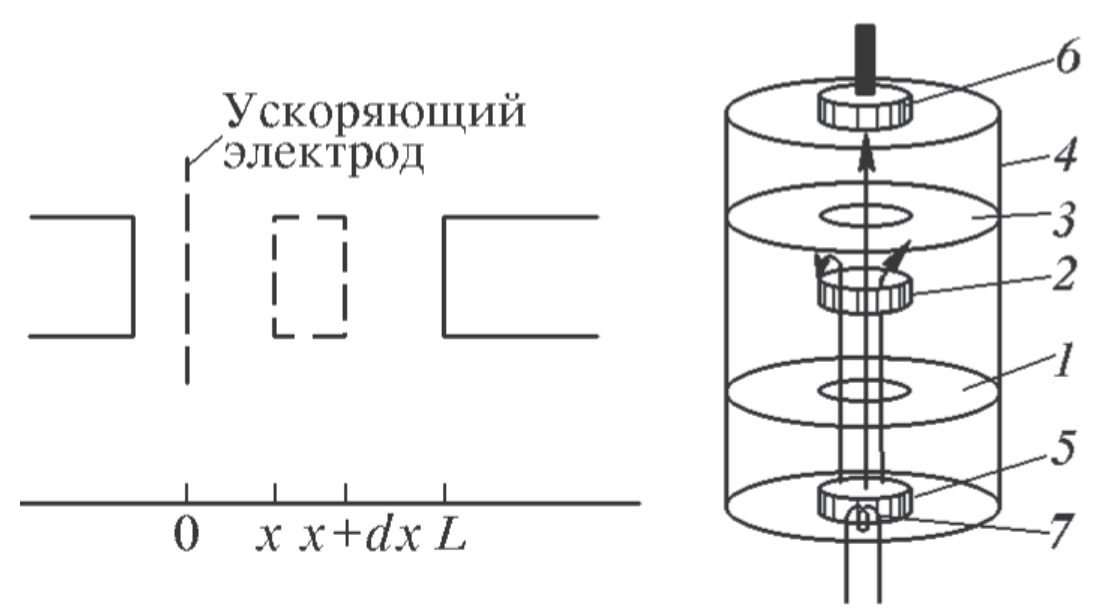
\includegraphics[width=0.8\textwidth]{res/3.png}
		\caption{Схематическое изображение тиратрона (слева) и его конструкция (справа): 1, 2, 3 — сетки; 4 — внешний металлический цилиндр; 5 — катод; 6 — анод; 7 — накаливаемая спираль}
	\end{wrapfigure}

	Электроны, эмитируемые катодом тиратрона, ускоряются напряжением $V$, приложенным между катодом и ближайшей к нему сеткой. Рассеянные электроны отклоняются в сторону и уходят на сетку, а оставшаяся часть электронов достигает анода и создает анодный ток $I_a$. Таким образом, поток электронов $N(x)$ на расстоянии $x$ от ускоряющей сетки уменьшается с ростом $x$ от начального значения $N_0$ у катода до некоторого
	значения $N_a$ у анода.
	
	Уравнение ВАХ:
	\begin{equation}
		I_a = I_0 e^{-C w(V)}, \;\; C = L n_a \Delta_a,
	\end{equation}
	где $I_0$ -- ток катода, $I_a$ -- анодный ток.
	
	Отсюда можно выразить:
	\begin{equation}
		w(V) = -\frac{1}{C} \ln\frac{I_a(V)}{I_0}.
		\label{w}
	\end{equation}
	
	\begin{figure}[h!]
		\centering
		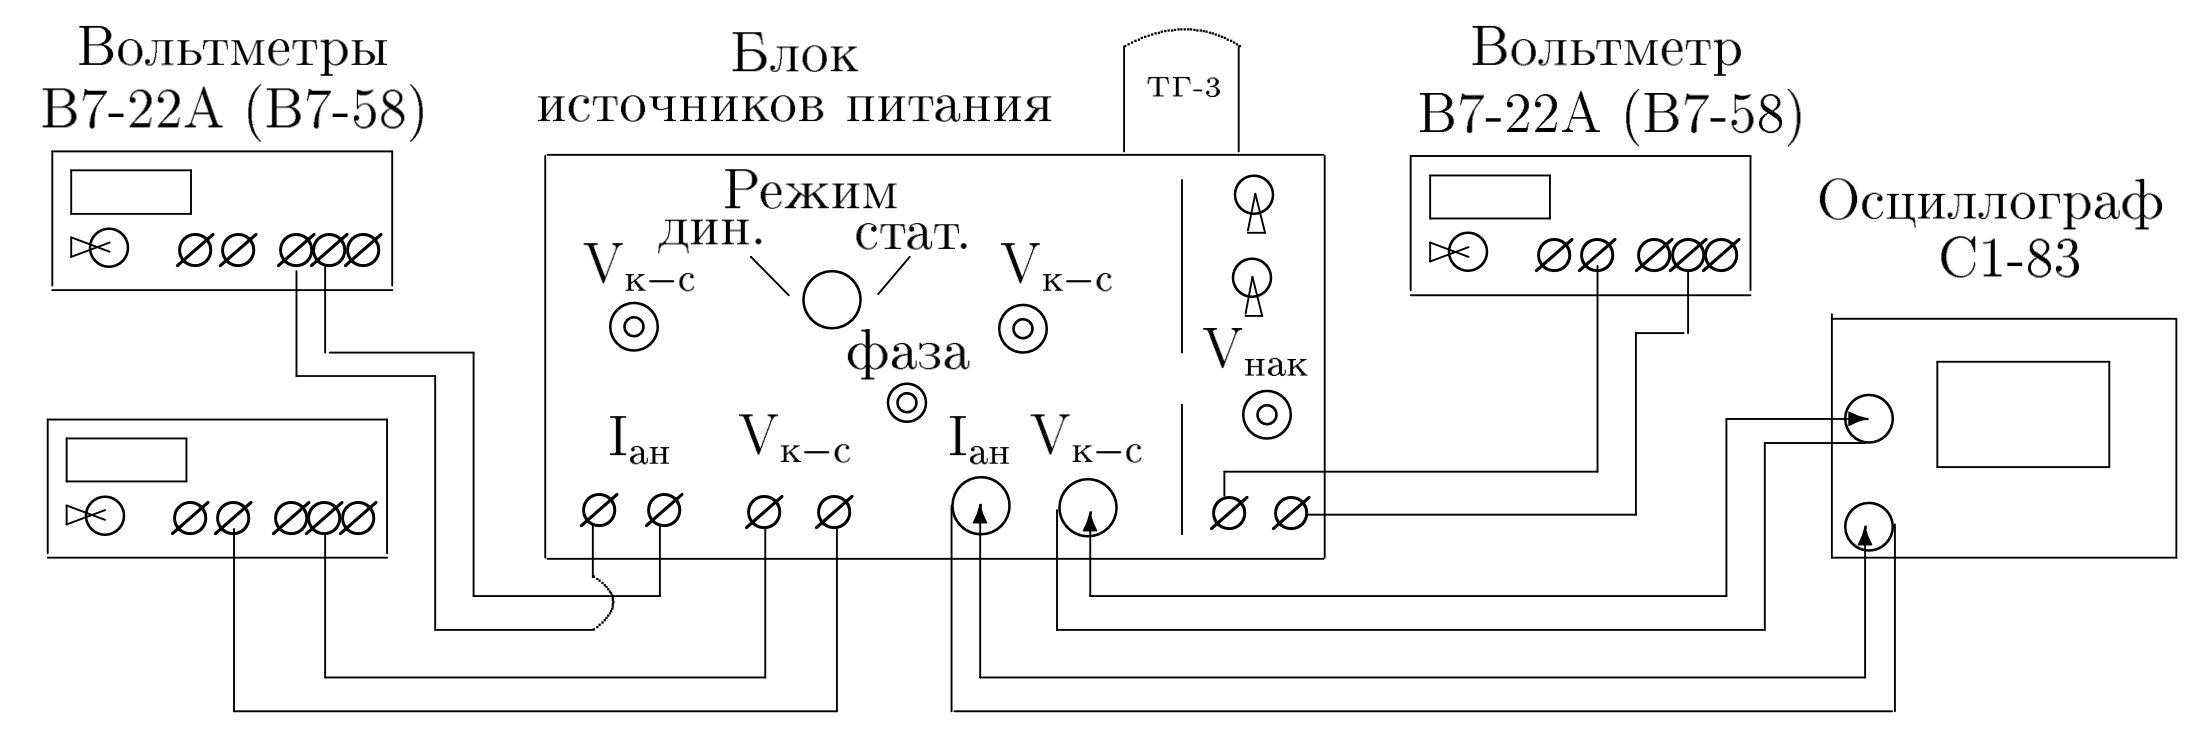
\includegraphics[width=1.0\linewidth]{res/4.png}
		\caption{Блок-схема экспериментальной установки}
	\end{figure}

\section*{Ход работы}

\begin{center}
		\textbf{I. Подготовка приборов к работе}
	\end{center}

	\begin{enumerate}
		\item Установим все ручки регулировки в крайнее левое положение.
		
		\item Убедимся, что все выходы подключены согласно схеме и включим осциллограф.
		
		\item На канале I установим ступенчатый переключатель в положение 0.2 V/дел, утопим соседнюю кнопку <<$\times$10>>, ручку плавного усиления повернем по часовой стрелке до щелчка.
		
		\item На канале II установим чувствительность 2 mV/дел $\times$ 10 = 20 mV/дел.
		
		\item Установим режим развертки.
		
		\item Установим закрытый вход на обоих каналах.
		
		\item Поместим луч на экране осциллографа чуть правее центра.
		
		\item Включим вольтметр.
	\end{enumerate}

	\begin{center}
		\textbf{II. Вольт-амперная характеристика тиратрона $I_a = f(U_c)$ на экране осциллографа С1-83}
	\end{center}

	\begin{enumerate}
		\item Установим динамический режим.
		
		\item Поставим напряжение накала $V = 2.61$ В. Погрешность $\sigma_U = 0.01$ В.
		
		\item Проследим за ходом ВАХ тиратрона при увеличении ускоряющего напряжения от 0 до максимума.
		
		\item Разместим картину в центре экрана.

		\begin{figure}[h!]
			\begin{minipage}[h]{0.49\linewidth}
				\center{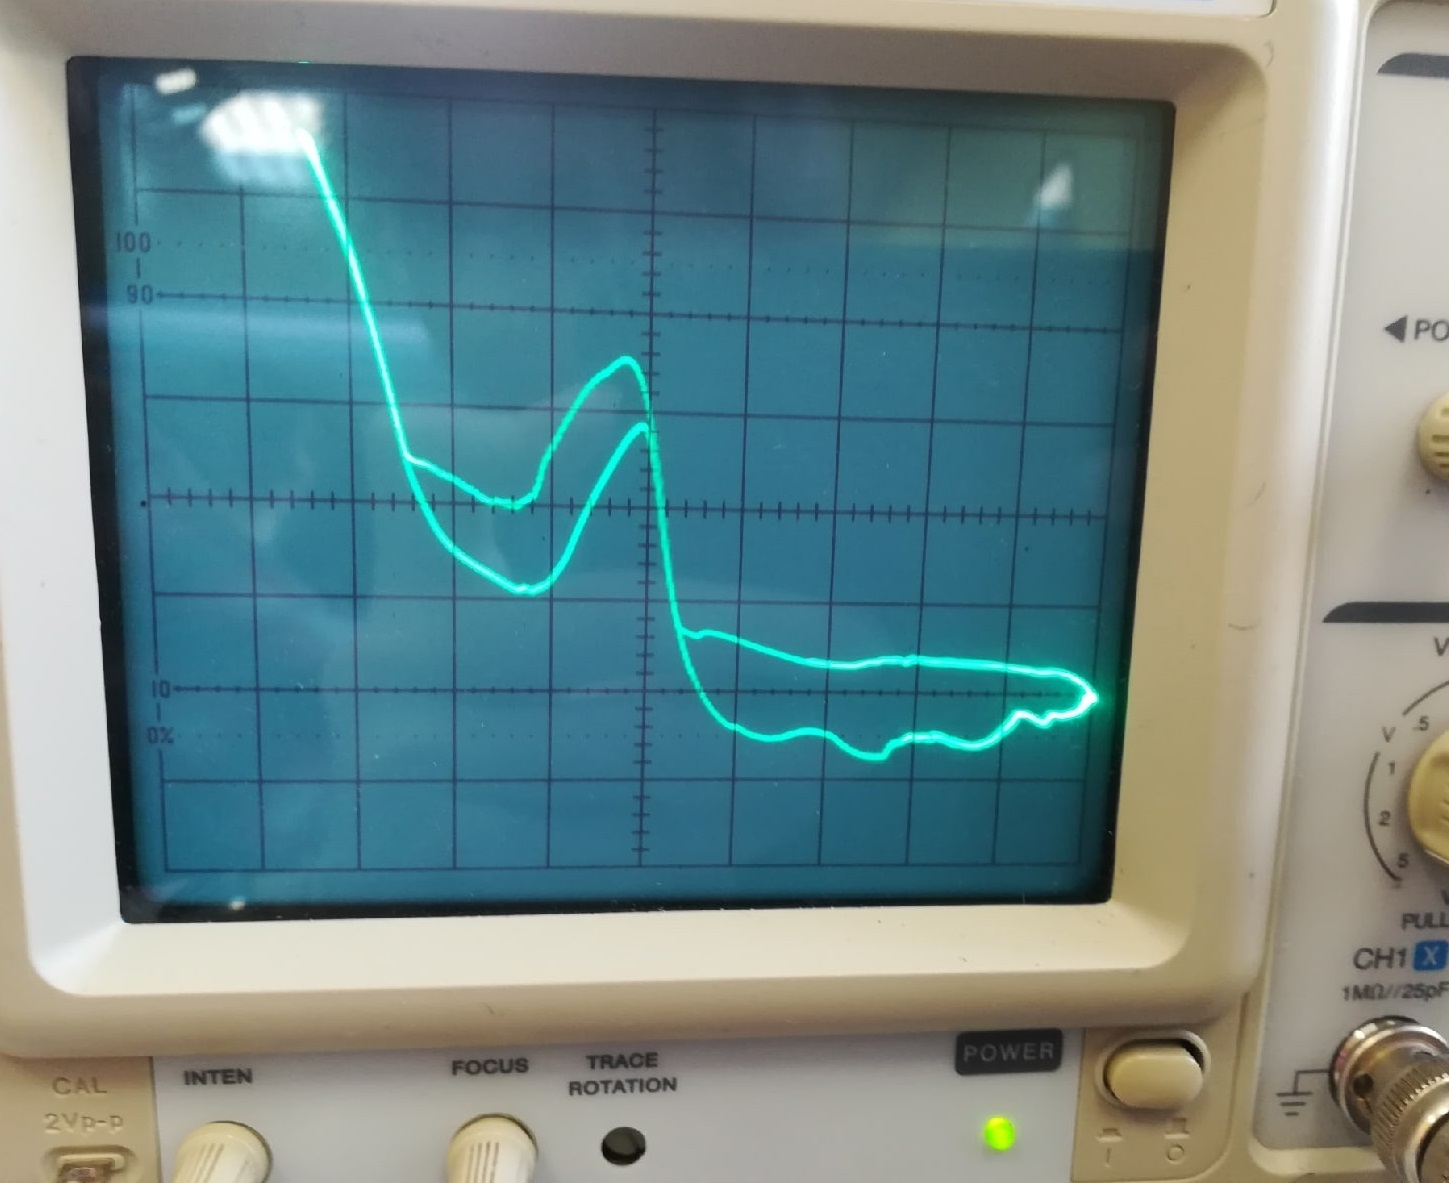
\includegraphics[width=1.02\linewidth]{src/5b.jpg}} \\ а\)}
			\end{minipage}
			\hfill
			\begin{minipage}[h]{0.49\linewidth}
				\center{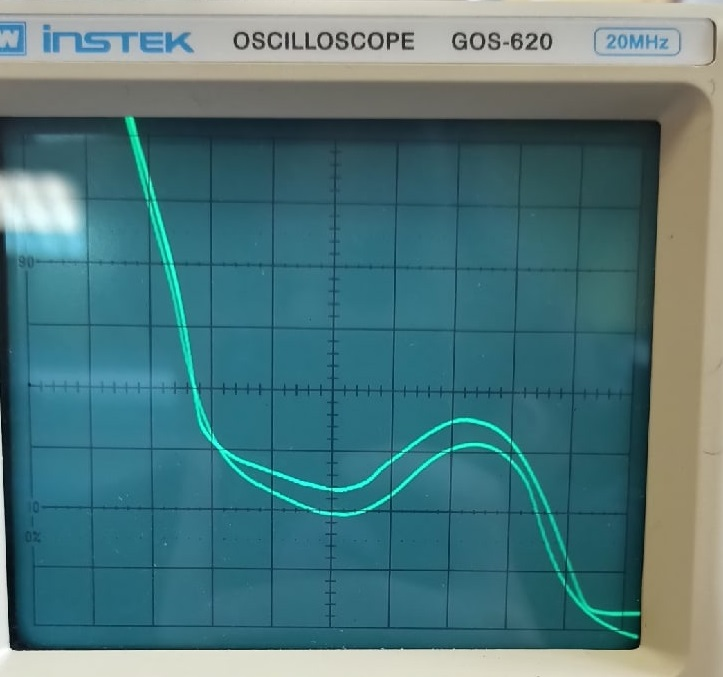
\includegraphics[width=0.9\linewidth]{src/5a.jpg}} \\ б)}
			\end{minipage}
			\caption{ВАХ тиратрона на экране осциллографа в динамическом режиме; a) при напряжении накала 2.61 В; б) при напряжении накала 2.97 В.}
		\end{figure}
	
		\item При максимальном ускоряющем напряжении измерим напряжения, соответствующие первому максимуму и первому минимуму, а также оценим напряжение пробоя. Результаты в запишем в таблицу 1.
		
		\item Повторим пункты 3--5 для напряжения накала $V = 2.97$ В.
		
		
		\begin{table}[h!]
			\centering
			\begin{tabular}{|ccc|}
				\hline
				\multicolumn{1}{|c|}{$V_{\text{max}}$, В} & \multicolumn{1}{c|}{$V_\text{min}$, В} & $V_\text{пробоя}$, В \\ \hline
				\multicolumn{3}{|c|}{$V_\text{накала} = 2.61$ В}                                                          \\ \hline
				\multicolumn{1}{|c|}{3.0}                 & \multicolumn{1}{c|}{7.0}              & 17.0                 \\ \hline
				\multicolumn{1}{|c|}{$V_{\text{max}}$, В} & \multicolumn{1}{c|}{$V_\text{min}$, В} & $V_\text{пробоя}$, В \\ \hline
				\multicolumn{3}{|c|}{$V_\text{накала} = 2.97$ В}                                                          \\ \hline
				\multicolumn{1}{|c|}{3.2}                 & \multicolumn{1}{c|}{8.2}              & 16.2                 \\ \hline
			\end{tabular}
			\caption{Измерения в динамическом режиме}
		\end{table}
		
		\item Поднесём к лампе магнит и пронаблюдаем за изменением ВАХ на экране осциллографа, так как он отклоняет электроны от своего пути.
	\end{enumerate}
	
	\begin{center}
		\textbf{III. Вольт-амперная характеристика $I_a = f(U_c)$ в статическом режиме}
	\end{center}

	\begin{enumerate}
		\item Установим статический режим.
		
		\item Включим режим измерения постоянного напряжения, проверим, что все клеммы подключены согласно схеме и включим вольтметр.
		
		\item Проведем измерение ВАХ тиратрона для тех же значений напряжений накала, что и в динамическом режиме. Ток анода определяется по показанию вольтметра $V_\text{анод-сетка}$, деленному на сопротивление 100 кОм, которое включено в цепь анода. Результаты запишем в таблицу 2.
		
		\begin{table}[h!]
			\centering
			\begin{tabular}{ccccc|lll|}
				\cline{1-3} \cline{6-8}
				\multicolumn{1}{|c|}{$V_\text{катод-сетка}$, В} & \multicolumn{1}{c|}{$V_\text{анод-сетка}$, В} & \multicolumn{1}{c|}{$I_a$, мА} &  &  & \multicolumn{1}{c|}{$V_\text{катод-сетка}$, В} & \multicolumn{1}{c|}{$V_\text{анод-сетка}$, В} & \multicolumn{1}{c|}{$I_a$, мА} \\ \cline{1-3} \cline{6-8} 
				\multicolumn{3}{|c|}{$V_\text{накала} = 2.61$ В}                                                                                 &  &  & \multicolumn{3}{c|}{$V_\text{накала} = 2.98$ В}                                                                                 \\ \cline{1-3} \cline{6-8} 
				\multicolumn{1}{|c|}{2.639}                     & \multicolumn{1}{c|}{2.95}                     & \multicolumn{1}{c|}{0.0295}    &  &  & \multicolumn{1}{l|}{2.979}                     & \multicolumn{1}{l|}{38.34}                    & 0.3834                         \\ \cline{1-3} \cline{6-8} 
				\multicolumn{1}{|c|}{3.162}                     & \multicolumn{1}{c|}{18.00}                       & \multicolumn{1}{c|}{0.1800}      &  &  & \multicolumn{1}{l|}{3.261}                     & \multicolumn{1}{l|}{47.71}                    & 0.4771                         \\ \cline{1-3} \cline{6-8} 
				\multicolumn{1}{|c|}{3.566}                     & \multicolumn{1}{c|}{21.60}                     & \multicolumn{1}{c|}{0.2160}     &  &  & \multicolumn{1}{l|}{3.514}                     & \multicolumn{1}{l|}{53.68}                    & 0.5368                         \\ \cline{1-3} \cline{6-8} 
				\multicolumn{1}{|c|}{4.111}                     & \multicolumn{1}{c|}{22.70}                     & \multicolumn{1}{c|}{0.2270}     &  &  & \multicolumn{1}{l|}{3.858}                     & \multicolumn{1}{l|}{60.01}                    & 0.6001                         \\ \cline{1-3} \cline{6-8} 
				\multicolumn{1}{|c|}{4.502}                     & \multicolumn{1}{c|}{22.75}                    & \multicolumn{1}{c|}{0.2275}    &  &  & \multicolumn{1}{l|}{4.045}                     & \multicolumn{1}{l|}{62.90}                     & 0.6290                          \\ \cline{1-3} \cline{6-8} 
				\multicolumn{1}{|c|}{5.299}                     & \multicolumn{1}{c|}{21.15}                    & \multicolumn{1}{c|}{0.2115}    &  &  & \multicolumn{1}{l|}{4.435}                     & \multicolumn{1}{l|}{67.51}                    & 0.6751                         \\ \cline{1-3} \cline{6-8} 
				\multicolumn{1}{|c|}{4.737}                     & \multicolumn{1}{c|}{22.88}                    & \multicolumn{1}{c|}{0.2288}    &  &  & \multicolumn{1}{l|}{5.028}                     & \multicolumn{1}{l|}{70.91}                    & 0.7091                         \\ \cline{1-3} \cline{6-8} 
				\multicolumn{1}{|c|}{6.325}                     & \multicolumn{1}{c|}{18.68}                    & \multicolumn{1}{c|}{0.1868}    &  &  & \multicolumn{1}{l|}{5.254}                     & \multicolumn{1}{l|}{71.45}                    & 0.7145                         \\ \cline{1-3} \cline{6-8} 
				\multicolumn{1}{|c|}{6.802}                     & \multicolumn{1}{c|}{17.18}                    & \multicolumn{1}{c|}{0.1718}    &  &  & \multicolumn{1}{l|}{5.424}                     & \multicolumn{1}{l|}{71.72}                    & 0.7172                         \\ \cline{1-3} \cline{6-8} 
				\multicolumn{1}{|c|}{7.095}                     & \multicolumn{1}{c|}{16.20}                     & \multicolumn{1}{c|}{0.1620}     &  &  & \multicolumn{1}{l|}{6.032}                     & \multicolumn{1}{l|}{71.23}                    & 0.7123                         \\ \cline{1-3} \cline{6-8} 
				\multicolumn{1}{|c|}{7.503}                     & \multicolumn{1}{c|}{14.72}                    & \multicolumn{1}{c|}{0.1472}    &  &  & \multicolumn{1}{l|}{6.248}                     & \multicolumn{1}{l|}{70.68}                    & 0.7068                         \\ \cline{1-3} \cline{6-8} 
				\multicolumn{1}{|c|}{8.232}                     & \multicolumn{1}{c|}{12.55}                    & \multicolumn{1}{c|}{0.1255}    &  &  & \multicolumn{1}{l|}{6.557}                     & \multicolumn{1}{l|}{69.29}                    & 0.6929                         \\ \cline{1-3} \cline{6-8} 
				\multicolumn{1}{|c|}{9.488}                     & \multicolumn{1}{c|}{10.25}                    & \multicolumn{1}{c|}{0.1025}    &  &  & \multicolumn{1}{l|}{6.730}                      & \multicolumn{1}{l|}{68.28}                    & 0.6828                         \\ \cline{1-3} \cline{6-8} 
				\multicolumn{1}{|c|}{10.625}                    & \multicolumn{1}{c|}{9.87}                     & \multicolumn{1}{c|}{0.0987}    &  &  & \multicolumn{1}{l|}{7.047}                     & \multicolumn{1}{l|}{65.89}                    & 0.6589                         \\ \cline{1-3} \cline{6-8} 
				\multicolumn{1}{|c|}{11.006}                    & \multicolumn{1}{c|}{10.09}                    & \multicolumn{1}{c|}{0.1009}    &  &  & \multicolumn{1}{l|}{7.472}                     & \multicolumn{1}{l|}{62.08}                    & 0.6208                         \\ \cline{1-3} \cline{6-8} 
				\multicolumn{1}{|c|}{11.588}                    & \multicolumn{1}{c|}{10.56}                    & \multicolumn{1}{c|}{0.1056}    &  &  & \multicolumn{1}{l|}{7.856}                     & \multicolumn{1}{l|}{58.62}                    & 0.5862                         \\ \cline{1-3} \cline{6-8} 
				\multicolumn{1}{|c|}{11.528}                    & \multicolumn{1}{c|}{10.52}                    & \multicolumn{1}{c|}{0.1052}    &  &  & \multicolumn{1}{l|}{8.712}                     & \multicolumn{1}{l|}{51.31}                    & 0.5131                         \\ \cline{1-3} \cline{6-8} 
				\multicolumn{1}{|c|}{12.197}                    & \multicolumn{1}{c|}{11.04}                    & \multicolumn{1}{c|}{0.1104}    &  &  & \multicolumn{1}{l|}{9.515}                     & \multicolumn{1}{l|}{46.82}                    & 0.4682                         \\ \cline{1-3} \cline{6-8} 
				\multicolumn{1}{|c|}{12.193}                    & \multicolumn{1}{c|}{11.06}                    & \multicolumn{1}{c|}{0.1106}    &  &  & \multicolumn{1}{l|}{10.394}                    & \multicolumn{1}{l|}{45.86}                    & 0.4586                         \\ \cline{1-3} \cline{6-8} 
				&                                               &                                &  &  & \multicolumn{1}{l|}{10.701}                    & \multicolumn{1}{l|}{46.52}                    & 0.4652                         \\ \cline{6-8} 
				&                                               &                                &  &  & \multicolumn{1}{l|}{11.280}                     & \multicolumn{1}{l|}{48.42}                    & 0.4842                         \\ \cline{6-8} 
				&                                               &                                &  &  & \multicolumn{1}{l|}{10.713}                    & \multicolumn{1}{l|}{46.85}                    & 0.4685                         \\ \cline{6-8} 
				&                                               &                                &  &  & \multicolumn{1}{l|}{10.850}                     & \multicolumn{1}{l|}{47.48}                    & 0.4748                         \\ \cline{6-8} 
			\end{tabular}
			\caption{Результаты измерений в статическом режиме}
		\end{table}
		
		\item По результатам измерений в динамическом режиме рассчитаем размер электронной оболочки атома инертного газа в опыте, приняв $U_0 = 2.5$ В.
		
		\textbf{Напряжение накала 2.61 В:}
		
		По формуле \eqref{E1}:
		\begin{equation*}
			l = \frac{1}{2}\frac{h}{\sqrt{2m(E_1 + U_0)}} \Longrightarrow l = (2.6 \pm 0.2) \text{ \AA}
		\end{equation*}
	
		По формуле \eqref{E2}:
		\begin{equation*}
			l = \frac{3}{4}\frac{h}{\sqrt{2m(E_2 + U_0)}} \Longrightarrow l = (3.0 \pm 0.1) \text{ \AA}
		\end{equation*}
	
		Исключив $U_0$ по формуле \eqref{E2E1}:
		\begin{equation*}
			l = (3.4 \pm 0.3) \text{ \AA}
		\end{equation*}
	
		Как видно, значения из разных опытов разнятся, но и погрешности достаточно велики. 
		
		Оценим глубину потенциальной ямы по формуле \eqref{U_0}:
		\begin{equation*}
			U_0 = (0.2 \pm 0.1) \text{ эВ}.
		\end{equation*}
	
		Глубина ямы получилась слишком неточной -- именно этот опыт мало, что может сказать нам о реальном значении.
		
		\textbf{Напряжение накала 2.97 В:}
		
		По формуле \eqref{E1}:
		\begin{equation*}
			l = \frac{1}{2}\frac{h}{\sqrt{2m(E_1 + U_0)}} \Longrightarrow l = (2.6 \pm 0.1) \text{ \AA}
		\end{equation*}
		
		По формуле \eqref{E2}:
		\begin{equation*}
			l = \frac{3}{4}\frac{h}{\sqrt{2m(E_2 + U_0)}} \Longrightarrow l = (2.8 \pm 0.1) \text{ \AA}
		\end{equation*}
		
		Исключив $U_0$ по формуле \eqref{E2E1}:
		\begin{equation*}
			l = (3.0 \pm 0.1) \text{ \AA}
		\end{equation*}
		
		Теперь значения получились более точными, и даже ближе друг к другу.
		
		Опять оценим глубину потенциальной ямы по формуле \eqref{U_0}:
		\begin{equation*}
			U_0 = (0.8 \pm 0.1) \text{ эВ}.
		\end{equation*}
		
		Гораздо лучше, однако далеко от совершенства, и значение ближе к предполагаемому 2.5 эВ.
		
		\item По результатам измерений напряжений пробоя оценим потенциал ионизации атома газа. В нашем случае получается:
		\begin{equation*}
			U = (16.6 \pm 0.6) \text{ эВ.} 
		\end{equation*}
	
		Данное значение близко к табличному для аргона $U_\text{табл} = 15.8$ эВ. Следовательно, делаем вывод, что в лампе аргон.
		
		\item Построим графики $I_a = f(V_c)$ для разных значений напряжений накала, опираясь на таблицу 2, и проведем те же расчеты, что и для динамического режима.
		
		\textbf{Напряжение накала 2.61 В:}
		\begin{figure}[h!]
			\centering
			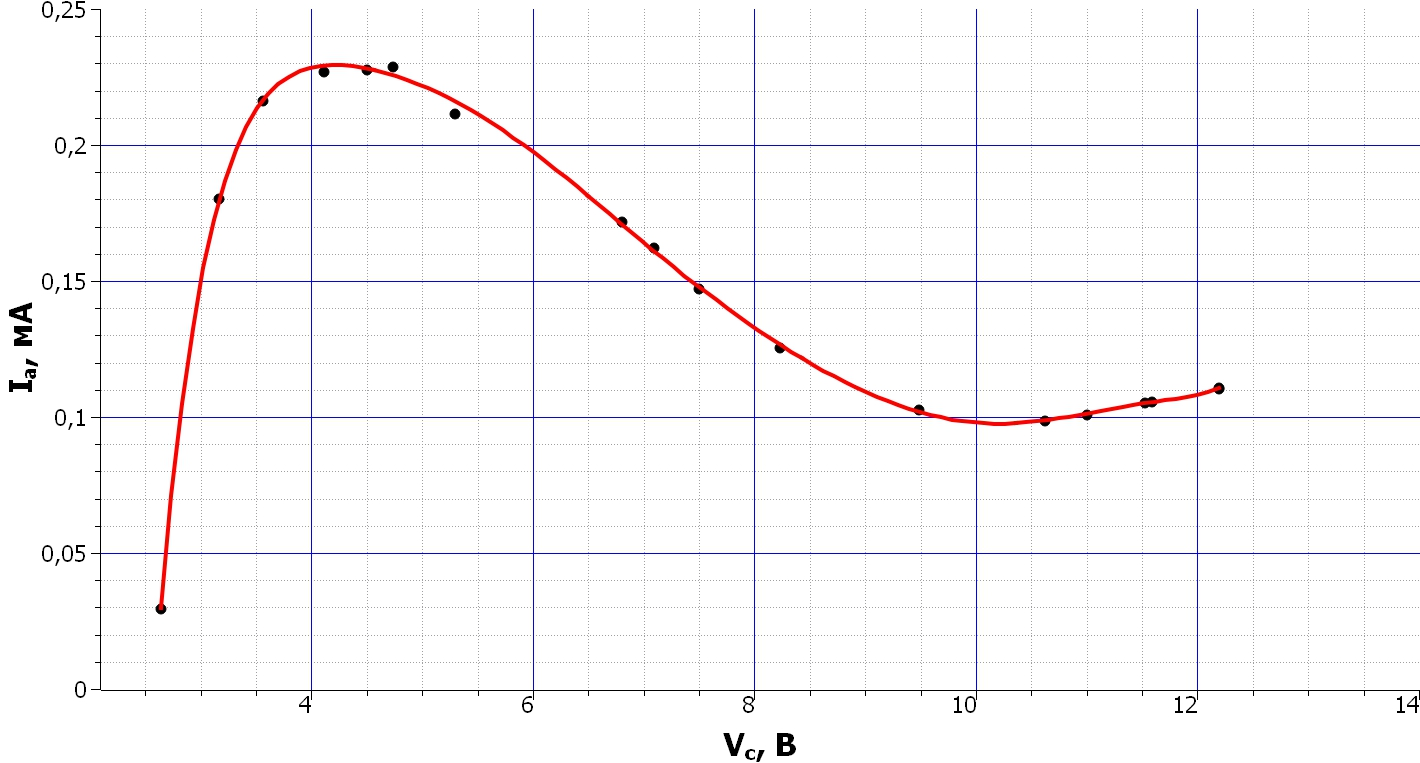
\includegraphics[width=\linewidth]{src/Ia(Vc)_261.jpg}
			\caption{Зависимость $I_a(V_c)$ для напряжения накала 2.61 В}
		\end{figure}
	
		$V_{max} = 4.1$ В, $V_{min} = 10.0$ В.
		
		Считаем размер электронной оболочки.
		
		По формуле \eqref{E1}:
		\begin{equation*}
			l = \frac{1}{2}\frac{h}{\sqrt{2m(E_1 + U_0)}} \Longrightarrow l = (2.4 \pm 0.1) \text{ \AA}
		\end{equation*}
		
		По формуле \eqref{E2}:
		\begin{equation*}
			l = \frac{3}{4}\frac{h}{\sqrt{2m(E_2 + U_0)}} \Longrightarrow l = (2.6 \pm 0.1) \text{ \AA}
		\end{equation*}
		
		Исключив $U_0$ по формуле \eqref{E2E1}:
		\begin{equation*}
			l = (2.8 \pm 0.2) \text{ \AA}
		\end{equation*}
	
		Видно, что на этот раз значения ближе друг к другу, и погрешности меньше.
	
		Оценим глубину потенциальной ямы по формуле \eqref{U_0}:
		\begin{equation*}
			U_0 = (0.60 \pm 0.03) \text{ эВ}.
		\end{equation*}
		
		С глубиной ямы тоже все получилось лучше, чем в динамическом случае.

	
		\textbf{Напряжение накала 2.98 В:}
		\begin{figure}[h!]
			\centering
			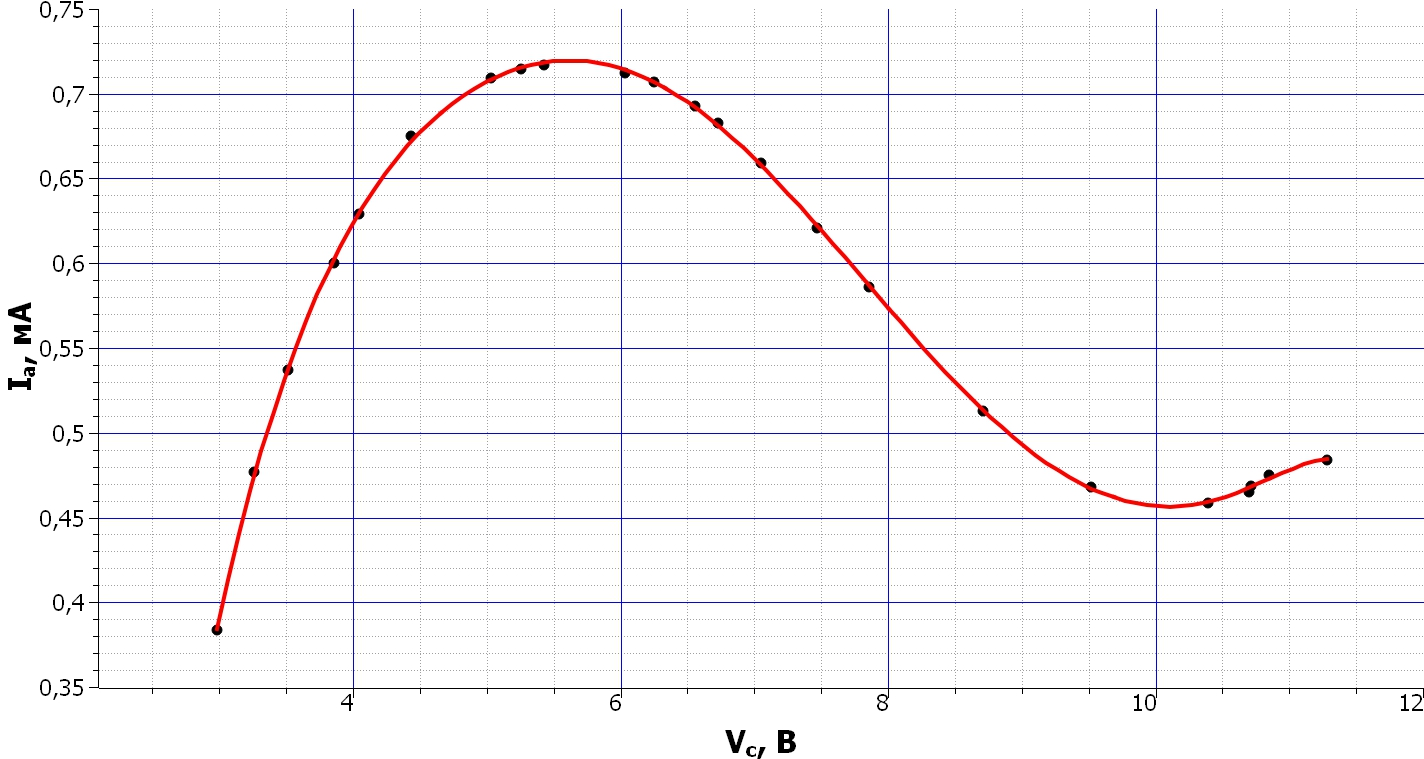
\includegraphics[width=\linewidth]{src/Ia(Vc)_298.jpg}
			\caption{Зависимость $I_a(V_c)$ для напряжения накала 2,98 В}
		\end{figure}
		
		$V_{max} = 5.5$ В, $V_{min} = 10.1$ В.
		
		Считаем размер электронной оболочки.
		
		По формуле \eqref{E1}:
		\begin{equation*}
			l = \frac{1}{2}\frac{h}{\sqrt{2m(E_1 + U_0)}} \Longrightarrow l = (2.2 \pm 0.1) \text{ \AA}
		\end{equation*}
		
		По формуле \eqref{E2}:
		\begin{equation*}
			l = \frac{3}{4}\frac{h}{\sqrt{2m(E_2 + U_0)}} \Longrightarrow l = (2.6 \pm 0.1) \text{ \AA}
		\end{equation*}
		
		Исключив $U_0$ по формуле \eqref{E2E1}:
		\begin{equation*}
			l = (3.2 \pm 0.1) \text{ \AA}
		\end{equation*}
		
		Этот случай чуть хуже, чем прошлый, но лишь тем, что значения получились разбросаны дальше.
		
		Оценить глубину потенциальной ямы в этом случае не представляется возможным, так как по формуле получается отрицательная величина. Однако она чрезвычайно мала по модулю, что говорит о том, что это результат погрешностей измерений.
	
		В итоге, среднее значение: $U_0^\Sigma = (0.53 \pm 0.14)$ эВ.
		И для размера электронной оболочки: $l^\Sigma = (2.8 \pm 0.5)$ \AA.
	
	
		\item Используя формулу \eqref{En}, оценим значения напряжений для максимумов при $n = 2.3$:
		\begin{equation*}
			E_n = \frac{(\pi n \hbar)^2}{2ml^2} - U_0.
		\end{equation*}
	
		$E_2^\text{max} \thicksim $ 18.7 эВ; $E_3^\text{max} \thicksim $ 42.8 эВ. 
	
		\item На основе формулы \eqref{w} найдем зависимость вероятности рассеяния электронов от энергии и построим график.
		\begin{equation*}
			Cw = \ln\frac{I_a(V)}{I_0}
		\end{equation*}
		
		И сам график выглядит так (ненормированный):
		\begin{figure}[h!]
			\centering
			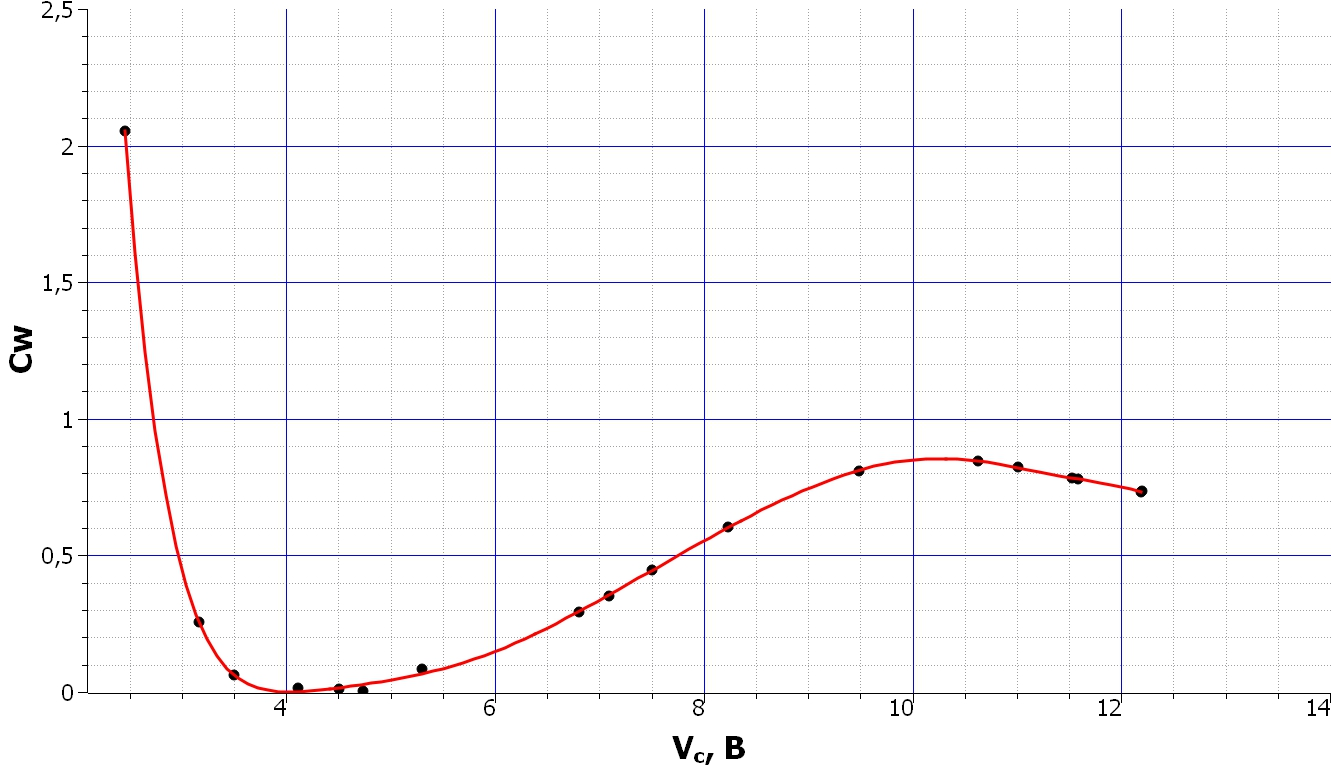
\includegraphics[width=\linewidth]{src/Cw(V).jpg}
			\caption{Зависимость вероятности рассеяния электронов}
		\end{figure}
	
	\end{enumerate}



\clearpage
    
\section*{Вывод}

В данной работе мы пронаблюдали эффект Рамзауэра. Было установлено, что в исследуемый инертный газ с высокой вероятностью является аргоном. Помимо этого, был оценен размер его внешней электронной оболочки: $l = (2.8 \pm 0.5)$ \AA. То же было проделано и с энергиями <<просветления>>: $E_2^\text{max} \thicksim $ 18.7 эВ; $E_3^\text{max} \thicksim $ 42.8 эВ. Была качественно установлена энергетическая зависимость вероятности рассеяния электронов на атомах аргона. Погрешности достаточно велики, что объясняется неточностью способа измерений. Свой вклад в погрешность вносит и методика измерений, и округление при расчетах. Именно поэтому полученные значения стоит рассматривать лишь как оценку искомых величин, а не непосредственно их истинные значения.

\vfill
    
\begin{thebibliography}{9}
	\bibitem{max} \emph{Лабораторный практикум по общей физике. В 3 томах. Том 3. Квантовая физика: учебное пособие} под ред. Ю. М. Ципенюка
\end{thebibliography}

\end{document}
